\subsubsection{Generazione automatica dello Swagger}
Per creare la documentazione dell'API è stata utilizzata la dipendenza \textit{springdoc-openapi-starter-webmvc-ui} citata nella sotto-sezione \hyperlink{doc-api}{4.7.2.1} nel capitolo di Progettazione. Grazie a questa dipendenza è stato possibile generare automaticamente la documentazione dell'API basata sulle annotazioni presenti nel codice sorgente. SpringDoc API utilizza le annotazioni di Spring per identificare i Controller, i metodi delle API, i dati in input e in output. Per visualizzare questo documento generato è possibile accederci tramite un endpoint specifico: \textit{https://localhost:porta\_scelta/swagger-ui.html}.
\begin{figure}[H] 
    \centering 
    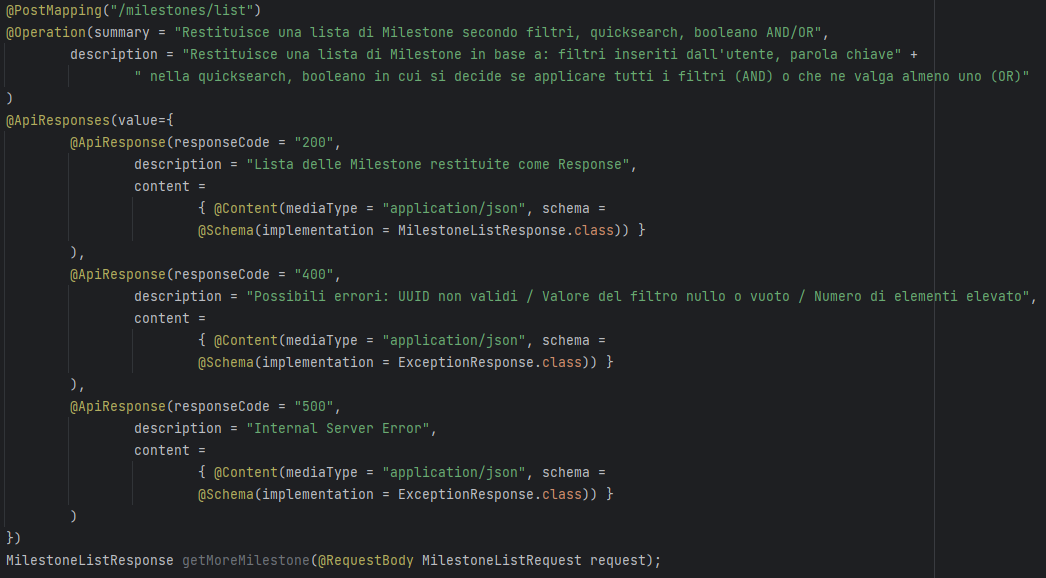
\includegraphics[width=1.00\columnwidth]{api-doc-annotazioni} 
    \caption{Annotazioni utili a generare la documentazione per l'API}
\end{figure}
\noindent La dipendenza importata fornisce anche annotazioni per arrichire il documento. In questa immagine notiamo le seguenti annotazioni:
\begin{itemize}
\item \textit{@Operation}, specifica un sommario dell'endpoint che l'utente può vedere prima di visualizzare nella sua totalità l'endpoint e un campo descrizione per fornire una descrizione più approfondita sul funzionamento;
\item \textit{@ApiResponses}, formata da tanti \textit{@ApiResponse} che specificano il codice di errore, la descrizione di quando questo errore esce e lo schema che avrà quando si presenterà.
\end{itemize}
Per agevolare la lettura dell'API è stata anche utilizzata la notazione \textit{@Schema} per fornire un nome appropriato a campi o classi.






